\chapter{FlowChart}

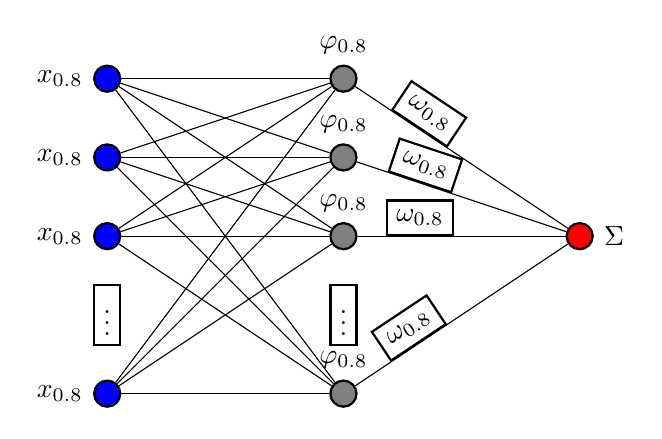
\begin{tikzpicture}
[   cnode/.style={draw=black,fill=#1,minimum width=3mm,circle},
]
    \node[cnode=red,label=0:$\Sigma$] (s) at (6,-3) {};
    \node at (0,-4) {$\vdots$};
    \node at (3,-4) {$\vdots$};
    \foreach \x in {1,...,4}
    {   \pgfmathparse{\x<4 ? \x : "n"}
        \node[cnode=blue,label=180:$x_{\pgfmathresult}$] (x-\x) at (0,{-\x-div(\x,4)}) {};
        \node[cnode=gray,label=90:$\varphi_{\pgfmathresult}$] (p-\x) at (3,{-\x-div(\x,4)}) {};
        \draw (p-\x) -- node[above,sloped,pos=0.3] {$\omega_{\pgfmathresult}$} (s);
    }
    \foreach \x in {1,...,4}
    {   \foreach \y in {1,...,4}
        {   \draw (x-\x) -- (p-\y);
        }
    }
\end{tikzpicture}

\definecolor{mybluei}{RGB}{124,156,205}
\definecolor{myblueii}{RGB}{73,121,193}
\definecolor{mygreen}{RGB}{202,217,126}
\definecolor{mypink}{RGB}{233,198,235}

\newcommand\widernode[5][widebox]{
  \node[
    #1,
    fit={(#2) (#3)},
    label=center:{\sffamily\bfseries\color{white}#4}] (#5) {};
}

\begin{tikzpicture}[node distance=3pt,outer sep=0pt,
    boxstyle/.style={
        draw=white,
        fill=#1,
        rounded corners,
        font={\sffamily\bfseries\color{white}},
        align=center,
        minimum height=30pt
    },
    box/.style={
        boxstyle=#1,
        text width=2cm},
        box/.default=mybluei,
        title/.style={font={\sffamily\bfseries\color{white}}},
        widebox/.style={draw=white,inner sep=0pt, rounded corners,fill=#1},
        widebox/.default=mybluei,
        mylabel/.style={font={\sffamily\bfseries\color{white}}},
]

\matrix (stack) [boxstyle=mybluei!40, draw=black,%  
column sep=3pt, row sep=3pt, inner sep=4mm,%
matrix of nodes,% 
nodes={box, outer sep=0pt, anchor=center, inner sep=3pt},%  
nodes in empty cells,
      row 1/.style={nodes={fill=none,draw=none,minimum height=3mm}},
] {
    &  & EPF Composer & & \\
        RCP main & Authoring & Browsing & Publishing & Search\\
        Rich Text & & &{XML\\ Export/Import} & MSP Export\\
        Common & & & & \\
        |[box=mypink]| Jtidy & & &|[box=mygreen]| GEF &|[box=mygreen]| ICU4J \\
        & & & & \\};

\widernode{stack-3-2}{stack-3-3}{Library Management}{LMg}
\widernode{stack-4-2}{stack-4-3}{UMA}{UMA}
\widernode{stack-4-4}{stack-4-5}{Export/Import}{ExImp}
\widernode[widebox=mygreen]{stack-5-2}{stack-5-3}{EMF}{EMF}
\widernode[widebox=mygreen]{stack-6-1}{stack-6-5}{RCP Runtime}{RCPrun}

\node [fit={(stack.south west)(stack.south east)},boxstyle=myblueii,draw=black,inner sep=0pt,below=3pt of stack.south,anchor=north,label={[mylabel]center:Java Runtime}] (JavaR) {};

\end{tikzpicture}

Some of the greatest \emph{discoveries} in science werer made by accident.

\textit{Some of the greatest \emph{discoveries} in science were made by accident.}

\textbf{Some of the greatest \emph{discoveries} in science were made by accident.}

In physics, the mass-energy equivalence is stated by the equation $E=mc^2$, discovered
in 1905 by Albert Einstein.

The mass-energy equivalence is described by the famous equation 

$$E=mc^2$$

discovered in 1905 by Albert Einstein.
In natural units($c = 1$), the formula expresses the identity

\begin{equation}
E=m
\end{equation}

Subscripts in math mode are written as $a_b$ and superscripts are written as $a^b$. 
These can be combined an nested to write expressions such as

$$T^{i_1 i_2 \dots i_p}_{j_1 j_2 \dots j_q} = T(x^{i_1},\dots,x^{i_p},e_{j_1},\dots,e_{j_q})$$

We write integrals using $\int$ and fractions using $\frac{a}{b}$. 
Limits are placed on integrals using superscripts and subscripts:

$$\int_0^1 \frac{1}{e^x} =  \frac{e-1}{e}$$

Lower case Greek letters are written as $\omega$ $\delta$ etc. 
while upper case Greek letters are written as $\Omega$ $\Delta$.

Mathematical operators are prefixed with a backslash as $\sin(\beta)$, $\cos(\alpha)$, $\log(x)$ etc.

% 流程图定义基本形状
\tikzstyle{startstop} = [rectangle, rounded corners, minimum width=3cm, minimum height=1cm,text centered, draw=black, fill=red!30]
\tikzstyle{io} = [trapezium, trapezium left angle=70, trapezium right angle=110, minimum width=3cm, minimum height=1cm, text centered, draw=black, fill=blue!30]
\tikzstyle{process} = [rectangle, minimum width=3cm, minimum height=1cm, text centered, draw=black, fill=orange!30]
\tikzstyle{decision} = [diamond, minimum width=3cm, minimum height=1cm, text centered, draw=black, fill=green!30]
\tikzstyle{arrow} = [thick,->,>=stealth]

\begin{tikzpicture}[node distance=2cm]
%定义流程图具体形状
\node (start) [startstop] {Start};
\node (in1) [io, below of=start] {Input};
\node (pro1) [process, below of=in1] {Process 1};
\node (dec1) [decision, below of=pro1, yshift=-0.5cm] {Decision 1};
\node (pro2a) [process, below of=dec1, yshift=-0.5cm] {Process 2a};
\node (pro2b) [process, right of=dec1, xshift=2cm] {Process 2b};
\node (out1) [io, below of=pro2a] {Output};
\node (stop) [startstop, below of=out1] {Stop};

%连接具体形状
\draw [arrow](start) -- (in1);
\draw [arrow](in1) -- (pro1);
\draw [arrow](pro1) -- (dec1);
\draw [arrow](dec1) -- (pro2a);
\draw [arrow](dec1) -- (pro2b);
\draw [arrow](dec1) -- node[anchor=east] {yes} (pro2a);
\draw [arrow](dec1) -- node[anchor=south] {no} (pro2b);
\draw [arrow](pro2b) |- (pro1);
\draw [arrow](pro2a) -- (out1);
\draw [arrow](out1) -- (stop);
\end{tikzpicture}

%作者:红伞菌
%链接:https://www.zhihu.com/question/20854046/answer/16400909
%来源:知乎
%著作权归作者所有。商业转载请联系作者获得授权,非商业转载请注明出处。
%作者:红伞菌
%链接:https://www.zhihu.com/question/20854046/answer/16400909
%来源:知乎
%著作权归作者所有。商业转载请联系作者获得授权,非商业转载请注明出处。

% Defines a `datastore' shape for use in DFDs.  This inherits from a
% rectangle and only draws two horizontal lines.
\makeatletter
\pgfdeclareshape{datastore}{
  \inheritsavedanchors[from=rectangle]
  \inheritanchorborder[from=rectangle]
  \inheritanchor[from=rectangle]{center}
  \inheritanchor[from=rectangle]{base}
  \inheritanchor[from=rectangle]{north}
  \inheritanchor[from=rectangle]{north east}
  \inheritanchor[from=rectangle]{east}
  \inheritanchor[from=rectangle]{south east}
  \inheritanchor[from=rectangle]{south}
  \inheritanchor[from=rectangle]{south west}
  \inheritanchor[from=rectangle]{west}
  \inheritanchor[from=rectangle]{north west}
  \backgroundpath{
    %  store lower right in xa/ya and upper right in xb/yb
    \southwest \pgf@xa=\pgf@x \pgf@ya=\pgf@y
    \northeast \pgf@xb=\pgf@x \pgf@yb=\pgf@y
    \pgfpathmoveto{\pgfpoint{\pgf@xa}{\pgf@ya}}
    \pgfpathlineto{\pgfpoint{\pgf@xb}{\pgf@ya}}
    \pgfpathmoveto{\pgfpoint{\pgf@xa}{\pgf@yb}}
    \pgfpathlineto{\pgfpoint{\pgf@xb}{\pgf@yb}}
 }
}
\makeatother
\begin{center}
\begin{tikzpicture}[
  font=\sffamily,
  every matrix/.style={ampersand replacement=\&,column sep=2cm,row sep=2cm},
  source/.style={draw,thick,rounded corners,fill=yellow!20,inner sep=.3cm},
  process/.style={draw,thick,circle,fill=blue!20},
  sink/.style={source,fill=green!20},
  datastore/.style={draw,very thick,shape=datastore,inner sep=.3cm},
  dots/.style={gray,scale=2},
  to/.style={->,>=stealth',shorten >=1pt,semithick,font=\sffamily\footnotesize},
  every node/.style={align=center}]

  % Position the nodes using a matrix layout
  \matrix{
    \node[source] (hisparcbox) {electronics};
      \& \node[process] (daq) {DAQ}; \& \\

    \& \node[datastore] (buffer) {buffer}; \& \\

    \node[datastore] (storage) {storage};
      \& \node[process] (monitor) {monitor};
      \& \node[sink] (datastore) {datastore}; \\
  };

  % Draw the arrows between the nodes and label them.
  \draw[to] (hisparcbox) -- node[midway,above] {raw events}
      node[midway,below] {level 0} (daq);
  \draw[to] (daq) -- node[midway,right] {raw event data\\level 1} (buffer);
  \draw[to] (buffer) --
      node[midway,right] {raw event data\\level 1} (monitor);
  \draw[to] (monitor) to[bend right=50] node[midway,above] {events}
      node[midway,below] {level 1} (storage);
  \draw[to] (storage) to[bend right=50] node[midway,above] {events}
      node[midway,below] {level 1} (monitor);
  \draw[to] (monitor) -- node[midway,above] {events}
      node[midway,below] {level 1} (datastore);
\end{tikzpicture}
\end{center}

\begin{figure}[htb]
\centering
%定义形状样式
\tikzstyle{startstop} = [rectangle, rounded corners, minimum width = 3cm, minimum height = 0.7cm, text centered, draw = black]
\tikzstyle{startstop2} = [rectangle, rounded corners, minimum width = 13cm, minimum height = 0.7cm, text centered, draw = black]
\tikzstyle{io} = [trapezium, trapezium left angle = 30, trapezium right angle = 150, minimum width = 3cm, text centered, draw = black, fill = white]
\tikzstyle{io2} = [trapezium, trapezium left angle = 30, trapezium right angle = 150, minimum width = 2.5cm, draw = black, fill = white]
\tikzstyle{io3} = [trapezium, trapezium left angle = 30, trapezium right angle = 150, minimum width = 2cm, draw = black, fill = white]
\tikzstyle{process} = [rectangle, minimum width = 3cm, minimum height = 1cm, text centered, draw = black]
\tikzstyle{decision} = [diamond, minimum width = 3cm, minimum height = 1cm, text centered, draw = black]
\tikzstyle{arrow} = [thick, -, >= stealth]
\tikzstyle{arrow2} = [thick, ->, >= stealth]

\begin{tikzpicture}[node distance = 1.5cm]
% 定义流程图具体形状
\coordinate[label = left:{\small 输入图像}](A) at(-1.5, 0);
\node(in1) [io] {};
\node(pro1) [startstop, below of = in1] {\small 线性滤波};

\node(in2 - 2)[io3, below of = pro1, yshift = -0.6cm]{};
\node(in3 - 2)[io3, left of = in2 - 2, xshift = -2.5cm]{};
\node(in4 - 2)[io3, right of = in2 - 2, xshift = 2.5cm]{};

\node(in2 - 1)[io2, below of = pro1, yshift = -0.3cm]{};
\node(in3 - 1)[io2, left of = in2 - 1, xshift = -2.5cm]{};
\node(in4 - 1)[io2, right of = in2 - 1, xshift = 2.5cm]{};

\node(in2) [io, below of = pro1] {\small 颜色};
\node(in3)[io, left of = in2, xshift = -2.5cm]{\small 亮度};
\node(in4)[io, right of = in2, xshift = 2.5cm]{\small 方向};

\node(in5)[startstop2, below of = in2 - 2]{\small Center - Surround差异计算及归一化};

\node(in6 - 2)[io3, below of = in5, yshift = -0.6cm]{};
\node(in7 - 2)[io3, left of = in6 - 2, xshift = -2.5cm]{};
\node(in8 - 2)[io3, right of = in6 - 2, xshift = 2.5cm]{};

\node(in6 - 1)[io2, below of = in5, yshift = -0.3cm]{};
\node(in7 - 1)[io2, left of = in6 - 1, xshift = -2.5cm]{};
\node(in8 - 1)[io2, right of = in6 - 1, xshift = 2.5cm]{};

\node(in6) [io, below of = in5] {};
\node(in7)[io, left of = in6, xshift = -2.5cm]{};
\node(in8)[io, right of = in6, xshift = 2.5cm]{};

\coordinate[label = left:{\small 特征图}](B) at(-1, -6.2);
\coordinate[label = left:{\small (12张)}](C) at(-1.5, -7.5);
\coordinate[label = left:{\small (6张)}](D) at(2.7, -7.5);
\coordinate[label = left:{\small (24张)}](E) at(6.7, -7.5);

\node(in9)[startstop2, below of = in6 - 2]{ \small 跨尺度合并及归一化 };

\node(in10) [io, below of = in9] {};
\node(in11)[io, left of = in10, xshift = -2.5cm]{};
\node(in12)[io, right of = in10, xshift = 2.5cm]{};

\coordinate[label = left:{\small 醒目图}](F) at(-1, -9.5);
\node(in13) [startstop, below of = in10] {\small 线性组合};
\node(in14) [io, below of = in13] {};
\coordinate[label = left:{\small 显著图}](G) at(-1, -13);

\node(in15) [startstop, below of = in14] {\small 赢者取全};
\coordinate[label = left:{\small 显著位置}]() at(1, -16.1);
\coordinate[label = left:{\small 反馈抑制}]() at(4.5, -14.7);

%连线
\draw[arrow](pro1) -- (in1);
\draw[arrow](pro1) -- (in2);
\draw[arrow](pro1) -- (in3);
\draw[arrow](pro1) -- (in4);
\draw[arrow](0, -4.75) -- (in2 - 2);
\draw[arrow](-4, -4.75) -- (in3 - 2);
\draw[arrow](4, -4.75) -- (in4 - 2);
\draw[arrow](0, -5.45) -- (in6);
\draw[arrow](-4, -5.45) -- (in7);
\draw[arrow](4, -5.45) -- (in8);
\draw[arrow](0, -8.35) -- (in6 - 2);
\draw[arrow](-4, -8.35) -- (in7 - 2);
\draw[arrow](4, -8.35) -- (in8 - 2);
\draw[arrow](0, -9.05) -- (in10);
\draw[arrow](-4, -9.05) -- (in11);
\draw[arrow](4, -9.05) -- (in12);
\draw[arrow](in13) -- (in10);
\draw[arrow](in13) -- (in11);
\draw[arrow](in13) -- (in12);
\draw[arrow](in13) -- (in14);
\draw[arrow](in14) -- (in15);
\draw[arrow](in15) -- (0, -15.8);
\draw[arrow](0, -15.4) -- (2.5, -15.4);
\draw[arrow](2.5, -14) -- (2.5, -15.4);
\draw[arrow2](2.5, -14) -- (0, -14);
\end{tikzpicture}
\caption{IT算法流程\cite{Itti}}
\end{figure}

% 设置颜色代号
\colorlet{lcfree}{green}
\colorlet{lcnorm}{blue}
\colorlet{lccong}{red}
% -------------------------------------------------
% 设置调试标志层
\pgfdeclarelayer{marx}
\pgfsetlayers{main,marx}
% 标记坐标点的宏定义。交换下面两个定义关闭。
\providecommand{\cmark}[2][]{%
  \begin{pgfonlayer}{marx}
    \node [nmark] at (c#2#1) {#2};
  \end{pgfonlayer}{marx}
  } 
\providecommand{\cmark}[2][]{\relax} 
% -------------------------------------------------
% 开始绘图
\begin{figure}[h]
\centering
\scalebox{.8}{                  %设置缩放	
\begin{tikzpicture}[
    >=triangle 60,              % 箭头的形状
    start chain=going below,    % 从上往下的流程
    node distance=6mm and 60mm, % 全局间距设置
    every join/.style={norm},   % 连接线的默认设置
    ]
% ------------------------------------------------- 
% 节点的样式定义 
% <on chain> 和 <on grid> 可以减少手动调整节点位置的麻烦
\tikzset{
  base/.style={draw, on chain, on grid, align=center, minimum height=4ex},
  proc/.style={base, rectangle, text width=8em},
  test/.style={base, diamond, aspect=2, text width=5em},
  term/.style={proc, rounded corners},
  % coord 用来表示连接线的转折点
  coord/.style={coordinate, on chain, on grid, node distance=6mm and 25mm},
  % nmark 用来表示调试标志
  nmark/.style={draw, cyan, circle, font={\sffamily\bfseries}},
  % -------------------------------------------------
  % 不同的连接线样式
  norm/.style={->, draw, lcnorm},
  free/.style={->, draw, lcfree},
  cong/.style={->, draw, lccong},
  it/.style={font={\small\itshape}}
}
% -------------------------------------------------
% 先放节点
\node [term, densely dotted,fill=lccong!25, it] (p0) {输入};
% 用 join 表示和上一个节点相连 
\node [proc, join]	{使用非线性最小二乘法得到 $X_0$};
\node [proc, join]	{记录 $X=X_0, f=f(X_0)$};
\node [test, join] (t1)	{$T>T_E$?};
\node [proc] (p1)		{$step=0$};
\node [test, join] (t2)	{$step<count$?};
\node [proc] (p2)		{得到新状态$P_N=P+scale\times rand$,计算目标函数差$\Delta f$};
\node [test, join] (t3)	{$F_{Accept}<rand$?};
\node [proc] (p3)		{记录新状态 $X=X_N,f=f(X_N)$};

\node [proc, left=of t1] (p4)	{$T=T\times a,scale=scale\times b$};
\node [term, densely dotted, right=of t1,fill=lcfree!25](p5)	{输出};
\node [proc, right=of t3](p6)	{$step++$};

\node [coord, left=of t2] (c1)  {}; 
\node [coord, right=of t2] (c2)  {}; 
\node [coord, right=of p3] (c3)  {}; 
%先画南北方向的连接线,先画线再画两端的标志和箭头
\path (t1.south) to node [near start, xshift=1em] {$y$} (p1);
  \draw [*->,lcnorm] (t1.south) -- (p1);
\path (t2.south) to node [near start, xshift=1em] {$y$} (p2);
  \draw [*->,lcnorm] (t2.south) -- (p2);
\path (t3.south) to node [near start, xshift=1em] {$y$} (p3);
  \draw [*->,lcnorm] (t3.south) -- (p3);
%接着画东西方向的连接线,方法同上
\path (t1.east) to node [near start, yshift=1em]  {$n$}(p5);
  \draw [o->,lcnorm] (t1.east) -- (p5);
  \draw [->,lcnorm] (p4.east) -- (t1);
\path (t3.east) to node [near start, yshift=1em]  {$n$}(p6);
  \draw [o->,lcnorm] (t3.east) -- (p6);
\path (t2.west) to node [near start, yshift=1em]  {$n$}(c1);
  \draw [o->,lcnorm] (t2.west) -- (c1) -| (p4);
  \draw [->,lcnorm] (p3.east) -- (c3) -| (p6.south);
  \draw [<-,lcnorm] (t2.east) -- (c2) -| (p6.north);
\end{tikzpicture}
}
\label{fig:algorithm}
\end{figure}

\tikzstyle{every node}=[draw=black,thick,anchor=west]
\tikzstyle{selected}=[draw=red,fill=red!30]
\tikzstyle{optional}=[dashed,fill=gray!50]
\begin{tikzpicture}[%
  grow via three points={one child at (0.5,-0.7) and
  two children at (0.5,-0.7) and (0.5,-1.4)},
  edge from parent path={(\tikzparentnode.south) |- (\tikzchildnode.west)}]
  \node {texmf}
    child { node {doc}}
    child { node {fonts}}
    child { node {source}}
    child { node [selected] {tex}
      child { node {generic}}
      child { node [optional] {latex}}
      child { node {plain}}
    }
    child [missing] {}
    child [missing] {}
    child [missing] {}
    child {node {texdoc}};
\end{tikzpicture}

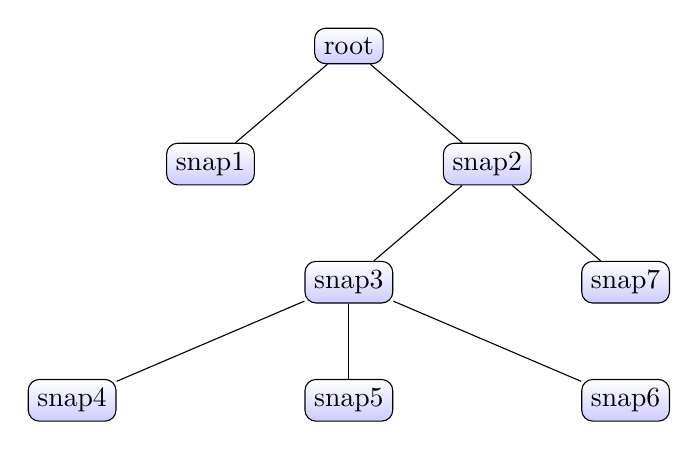
\begin{tikzpicture}[sibling distance=10em,
    every node/.style = {shape=rectangle, rounded corners,
        draw, align=center,
        top color=white, bottom color=blue!20}]]
        \node {root}
        child { node {snap1} }
        child { node {snap2}
            child { node {snap3}
                child { node {snap4} }
                child { node {snap5} }
                child { node {snap6} } }
            child { node {snap7} } };
\end{tikzpicture}

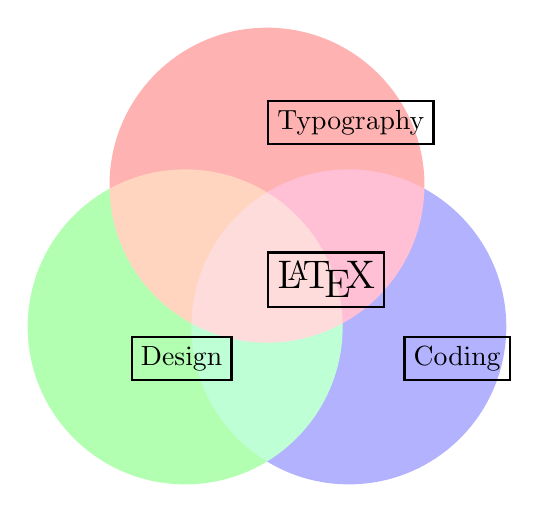
\begin{tikzpicture}
  \begin{scope}[blend group = soft light]
    \fill[red!30!white]   ( 90:1.2) circle (2);
    \fill[green!30!white] (210:1.2) circle (2);
    \fill[blue!30!white]  (330:1.2) circle (2);
  \end{scope}
  \node at ( 90:2)    {Typography};
  \node at ( 210:2)   {Design};
  \node at ( 330:2)   {Coding};
  \node [font=\Large] {\LaTeX};
\end{tikzpicture}

% Drawing part, node distance is 1.5 cm and every node
% is prefilled with white background
\begin{tikzpicture}[node distance=1.5cm,
    every node/.style={fill=white, font=\sffamily}, align=center]
  % Specification of nodes (position, etc.)
  \node (start)             [activityStarts]              {Activity starts};
  \node (onCreateBlock)     [process, below of=start]          {onCreate()};
  \node (onStartBlock)      [process, below of=onCreateBlock]   {onStart()};
  \node (onResumeBlock)     [process, below of=onStartBlock]   {onResume()};
  \node (activityRuns)      [activityRuns, below of=onResumeBlock]
                                                      {Activity is running};
  \node (onPauseBlock)      [process, below of=activityRuns, yshift=-1cm]
                                                                {onPause()};
  \node (onStopBlock)       [process, below of=onPauseBlock, yshift=-1cm]
                                                                 {onStop()};
  \node (onDestroyBlock)    [process, below of=onStopBlock, yshift=-1cm] 
                                                              {onDestroy()};
  \node (onRestartBlock)    [process, right of=onStartBlock, xshift=4cm]
                                                              {onRestart()};
  \node (ActivityEnds)      [startstop, left of=activityRuns, xshift=-4cm]
                                                        {Process is killed};
  \node (ActivityDestroyed) [startstop, below of=onDestroyBlock]
                                                    {Activity is shut down};     
  % Specification of lines between nodes specified above
  % with aditional nodes for description 
  \draw[->]             (start) -- (onCreateBlock);
  \draw[->]     (onCreateBlock) -- (onStartBlock);
  \draw[->]      (onStartBlock) -- (onResumeBlock);
  \draw[->]     (onResumeBlock) -- (activityRuns);
  \draw[->]      (activityRuns) -- node[text width=4cm]
                                   {Another activity comes in
                                    front of the activity} (onPauseBlock);
  \draw[->]      (onPauseBlock) -- node {The activity is no longer visible}
                                   (onStopBlock);
  \draw[->]       (onStopBlock) -- node {The activity is shut down by
                                   user or system} (onDestroyBlock);
  \draw[->]    (onRestartBlock) -- (onStartBlock);
  \draw[->]       (onStopBlock) -| node[yshift=1.25cm, text width=3cm]
                                   {The activity comes to the foreground}
                                   (onRestartBlock);
  \draw[->]    (onDestroyBlock) -- (ActivityDestroyed);
  \draw[->]      (onPauseBlock) -| node(priorityXMemory)
                                   {higher priority $\rightarrow$ more memory}
                                   (ActivityEnds);
  \draw           (onStopBlock) -| (priorityXMemory);
  \draw[->]     (ActivityEnds)  |- node [yshift=-2cm, text width=3.1cm]
                                    {User navigates back to the activity}
                                    (onCreateBlock);
  \draw[->] (onPauseBlock.east) -- ++(2.6,0) -- ++(0,2) -- ++(0,2) --                
     node[xshift=1.2cm,yshift=-1.5cm, text width=2.5cm]
     {The activity comes to the foreground}(onResumeBlock.east);
\end{tikzpicture}
